\documentclass[11pt]{article}

    \usepackage[breakable]{tcolorbox}
    \usepackage{parskip} % Stop auto-indenting (to mimic markdown behaviour)
    

    % Basic figure setup, for now with no caption control since it's done
    % automatically by Pandoc (which extracts ![](path) syntax from Markdown).
    \usepackage{graphicx}
    % Maintain compatibility with old templates. Remove in nbconvert 6.0
    \let\Oldincludegraphics\includegraphics
    % Ensure that by default, figures have no caption (until we provide a
    % proper Figure object with a Caption API and a way to capture that
    % in the conversion process - todo).
    \usepackage{caption}
    \DeclareCaptionFormat{nocaption}{}
    \captionsetup{format=nocaption,aboveskip=0pt,belowskip=0pt}

    \usepackage{float}
    \floatplacement{figure}{H} % forces figures to be placed at the correct location
    \usepackage{xcolor} % Allow colors to be defined
    \usepackage{enumerate} % Needed for markdown enumerations to work
    \usepackage{geometry} % Used to adjust the document margins
    \usepackage{amsmath} % Equations
    \usepackage{amssymb} % Equations
    \usepackage{textcomp} % defines textquotesingle
    % Hack from http://tex.stackexchange.com/a/47451/13684:
    \AtBeginDocument{%
        \def\PYZsq{\textquotesingle}% Upright quotes in Pygmentized code
    }
    \usepackage{upquote} % Upright quotes for verbatim code
    \usepackage{eurosym} % defines \euro

    \usepackage{iftex}
    \ifPDFTeX
        \usepackage[T1]{fontenc}
        \IfFileExists{alphabeta.sty}{
              \usepackage{alphabeta}
          }{
              \usepackage[mathletters]{ucs}
              \usepackage[utf8x]{inputenc}
          }
    \else
        \usepackage{fontspec}
        \usepackage{unicode-math}
    \fi

    \usepackage{fancyvrb} % verbatim replacement that allows latex
    \usepackage{grffile} % extends the file name processing of package graphics
                         % to support a larger range
    \makeatletter % fix for old versions of grffile with XeLaTeX
    \@ifpackagelater{grffile}{2019/11/01}
    {
      % Do nothing on new versions
    }
    {
      \def\Gread@@xetex#1{%
        \IfFileExists{"\Gin@base".bb}%
        {\Gread@eps{\Gin@base.bb}}%
        {\Gread@@xetex@aux#1}%
      }
    }
    \makeatother
    \usepackage[Export]{adjustbox} % Used to constrain images to a maximum size
    \adjustboxset{max size={0.9\linewidth}{0.9\paperheight}}

    % The hyperref package gives us a pdf with properly built
    % internal navigation ('pdf bookmarks' for the table of contents,
    % internal cross-reference links, web links for URLs, etc.)
    \usepackage{hyperref}
    % The default LaTeX title has an obnoxious amount of whitespace. By default,
    % titling removes some of it. It also provides customization options.
    \usepackage{titling}
    \usepackage{longtable} % longtable support required by pandoc >1.10
    \usepackage{booktabs}  % table support for pandoc > 1.12.2
    \usepackage{array}     % table support for pandoc >= 2.11.3
    \usepackage{calc}      % table minipage width calculation for pandoc >= 2.11.1
    \usepackage[inline]{enumitem} % IRkernel/repr support (it uses the enumerate* environment)
    \usepackage[normalem]{ulem} % ulem is needed to support strikethroughs (\sout)
                                % normalem makes italics be italics, not underlines
    \usepackage{soul}      % strikethrough (\st) support for pandoc >= 3.0.0
    \usepackage{mathrsfs}
    

    
    % Colors for the hyperref package
    \definecolor{urlcolor}{rgb}{0,.145,.698}
    \definecolor{linkcolor}{rgb}{.71,0.21,0.01}
    \definecolor{citecolor}{rgb}{.12,.54,.11}

    % ANSI colors
    \definecolor{ansi-black}{HTML}{3E424D}
    \definecolor{ansi-black-intense}{HTML}{282C36}
    \definecolor{ansi-red}{HTML}{E75C58}
    \definecolor{ansi-red-intense}{HTML}{B22B31}
    \definecolor{ansi-green}{HTML}{00A250}
    \definecolor{ansi-green-intense}{HTML}{007427}
    \definecolor{ansi-yellow}{HTML}{DDB62B}
    \definecolor{ansi-yellow-intense}{HTML}{B27D12}
    \definecolor{ansi-blue}{HTML}{208FFB}
    \definecolor{ansi-blue-intense}{HTML}{0065CA}
    \definecolor{ansi-magenta}{HTML}{D160C4}
    \definecolor{ansi-magenta-intense}{HTML}{A03196}
    \definecolor{ansi-cyan}{HTML}{60C6C8}
    \definecolor{ansi-cyan-intense}{HTML}{258F8F}
    \definecolor{ansi-white}{HTML}{C5C1B4}
    \definecolor{ansi-white-intense}{HTML}{A1A6B2}
    \definecolor{ansi-default-inverse-fg}{HTML}{FFFFFF}
    \definecolor{ansi-default-inverse-bg}{HTML}{000000}

    % common color for the border for error outputs.
    \definecolor{outerrorbackground}{HTML}{FFDFDF}

    % commands and environments needed by pandoc snippets
    % extracted from the output of `pandoc -s`
    \providecommand{\tightlist}{%
      \setlength{\itemsep}{0pt}\setlength{\parskip}{0pt}}
    \DefineVerbatimEnvironment{Highlighting}{Verbatim}{commandchars=\\\{\}}
    % Add ',fontsize=\small' for more characters per line
    \newenvironment{Shaded}{}{}
    \newcommand{\KeywordTok}[1]{\textcolor[rgb]{0.00,0.44,0.13}{\textbf{{#1}}}}
    \newcommand{\DataTypeTok}[1]{\textcolor[rgb]{0.56,0.13,0.00}{{#1}}}
    \newcommand{\DecValTok}[1]{\textcolor[rgb]{0.25,0.63,0.44}{{#1}}}
    \newcommand{\BaseNTok}[1]{\textcolor[rgb]{0.25,0.63,0.44}{{#1}}}
    \newcommand{\FloatTok}[1]{\textcolor[rgb]{0.25,0.63,0.44}{{#1}}}
    \newcommand{\CharTok}[1]{\textcolor[rgb]{0.25,0.44,0.63}{{#1}}}
    \newcommand{\StringTok}[1]{\textcolor[rgb]{0.25,0.44,0.63}{{#1}}}
    \newcommand{\CommentTok}[1]{\textcolor[rgb]{0.38,0.63,0.69}{\textit{{#1}}}}
    \newcommand{\OtherTok}[1]{\textcolor[rgb]{0.00,0.44,0.13}{{#1}}}
    \newcommand{\AlertTok}[1]{\textcolor[rgb]{1.00,0.00,0.00}{\textbf{{#1}}}}
    \newcommand{\FunctionTok}[1]{\textcolor[rgb]{0.02,0.16,0.49}{{#1}}}
    \newcommand{\RegionMarkerTok}[1]{{#1}}
    \newcommand{\ErrorTok}[1]{\textcolor[rgb]{1.00,0.00,0.00}{\textbf{{#1}}}}
    \newcommand{\NormalTok}[1]{{#1}}

    % Additional commands for more recent versions of Pandoc
    \newcommand{\ConstantTok}[1]{\textcolor[rgb]{0.53,0.00,0.00}{{#1}}}
    \newcommand{\SpecialCharTok}[1]{\textcolor[rgb]{0.25,0.44,0.63}{{#1}}}
    \newcommand{\VerbatimStringTok}[1]{\textcolor[rgb]{0.25,0.44,0.63}{{#1}}}
    \newcommand{\SpecialStringTok}[1]{\textcolor[rgb]{0.73,0.40,0.53}{{#1}}}
    \newcommand{\ImportTok}[1]{{#1}}
    \newcommand{\DocumentationTok}[1]{\textcolor[rgb]{0.73,0.13,0.13}{\textit{{#1}}}}
    \newcommand{\AnnotationTok}[1]{\textcolor[rgb]{0.38,0.63,0.69}{\textbf{\textit{{#1}}}}}
    \newcommand{\CommentVarTok}[1]{\textcolor[rgb]{0.38,0.63,0.69}{\textbf{\textit{{#1}}}}}
    \newcommand{\VariableTok}[1]{\textcolor[rgb]{0.10,0.09,0.49}{{#1}}}
    \newcommand{\ControlFlowTok}[1]{\textcolor[rgb]{0.00,0.44,0.13}{\textbf{{#1}}}}
    \newcommand{\OperatorTok}[1]{\textcolor[rgb]{0.40,0.40,0.40}{{#1}}}
    \newcommand{\BuiltInTok}[1]{{#1}}
    \newcommand{\ExtensionTok}[1]{{#1}}
    \newcommand{\PreprocessorTok}[1]{\textcolor[rgb]{0.74,0.48,0.00}{{#1}}}
    \newcommand{\AttributeTok}[1]{\textcolor[rgb]{0.49,0.56,0.16}{{#1}}}
    \newcommand{\InformationTok}[1]{\textcolor[rgb]{0.38,0.63,0.69}{\textbf{\textit{{#1}}}}}
    \newcommand{\WarningTok}[1]{\textcolor[rgb]{0.38,0.63,0.69}{\textbf{\textit{{#1}}}}}


    % Define a nice break command that doesn't care if a line doesn't already
    % exist.
    \def\br{\hspace*{\fill} \\* }
    % Math Jax compatibility definitions
    \def\gt{>}
    \def\lt{<}
    \let\Oldtex\TeX
    \let\Oldlatex\LaTeX
    \renewcommand{\TeX}{\textrm{\Oldtex}}
    \renewcommand{\LaTeX}{\textrm{\Oldlatex}}
    % Document parameters
    % Document title
    \title{Tarea 1}
    
    
    
    
    
    
    
% Pygments definitions
\makeatletter
\def\PY@reset{\let\PY@it=\relax \let\PY@bf=\relax%
    \let\PY@ul=\relax \let\PY@tc=\relax%
    \let\PY@bc=\relax \let\PY@ff=\relax}
\def\PY@tok#1{\csname PY@tok@#1\endcsname}
\def\PY@toks#1+{\ifx\relax#1\empty\else%
    \PY@tok{#1}\expandafter\PY@toks\fi}
\def\PY@do#1{\PY@bc{\PY@tc{\PY@ul{%
    \PY@it{\PY@bf{\PY@ff{#1}}}}}}}
\def\PY#1#2{\PY@reset\PY@toks#1+\relax+\PY@do{#2}}

\@namedef{PY@tok@w}{\def\PY@tc##1{\textcolor[rgb]{0.73,0.73,0.73}{##1}}}
\@namedef{PY@tok@c}{\let\PY@it=\textit\def\PY@tc##1{\textcolor[rgb]{0.24,0.48,0.48}{##1}}}
\@namedef{PY@tok@cp}{\def\PY@tc##1{\textcolor[rgb]{0.61,0.40,0.00}{##1}}}
\@namedef{PY@tok@k}{\let\PY@bf=\textbf\def\PY@tc##1{\textcolor[rgb]{0.00,0.50,0.00}{##1}}}
\@namedef{PY@tok@kp}{\def\PY@tc##1{\textcolor[rgb]{0.00,0.50,0.00}{##1}}}
\@namedef{PY@tok@kt}{\def\PY@tc##1{\textcolor[rgb]{0.69,0.00,0.25}{##1}}}
\@namedef{PY@tok@o}{\def\PY@tc##1{\textcolor[rgb]{0.40,0.40,0.40}{##1}}}
\@namedef{PY@tok@ow}{\let\PY@bf=\textbf\def\PY@tc##1{\textcolor[rgb]{0.67,0.13,1.00}{##1}}}
\@namedef{PY@tok@nb}{\def\PY@tc##1{\textcolor[rgb]{0.00,0.50,0.00}{##1}}}
\@namedef{PY@tok@nf}{\def\PY@tc##1{\textcolor[rgb]{0.00,0.00,1.00}{##1}}}
\@namedef{PY@tok@nc}{\let\PY@bf=\textbf\def\PY@tc##1{\textcolor[rgb]{0.00,0.00,1.00}{##1}}}
\@namedef{PY@tok@nn}{\let\PY@bf=\textbf\def\PY@tc##1{\textcolor[rgb]{0.00,0.00,1.00}{##1}}}
\@namedef{PY@tok@ne}{\let\PY@bf=\textbf\def\PY@tc##1{\textcolor[rgb]{0.80,0.25,0.22}{##1}}}
\@namedef{PY@tok@nv}{\def\PY@tc##1{\textcolor[rgb]{0.10,0.09,0.49}{##1}}}
\@namedef{PY@tok@no}{\def\PY@tc##1{\textcolor[rgb]{0.53,0.00,0.00}{##1}}}
\@namedef{PY@tok@nl}{\def\PY@tc##1{\textcolor[rgb]{0.46,0.46,0.00}{##1}}}
\@namedef{PY@tok@ni}{\let\PY@bf=\textbf\def\PY@tc##1{\textcolor[rgb]{0.44,0.44,0.44}{##1}}}
\@namedef{PY@tok@na}{\def\PY@tc##1{\textcolor[rgb]{0.41,0.47,0.13}{##1}}}
\@namedef{PY@tok@nt}{\let\PY@bf=\textbf\def\PY@tc##1{\textcolor[rgb]{0.00,0.50,0.00}{##1}}}
\@namedef{PY@tok@nd}{\def\PY@tc##1{\textcolor[rgb]{0.67,0.13,1.00}{##1}}}
\@namedef{PY@tok@s}{\def\PY@tc##1{\textcolor[rgb]{0.73,0.13,0.13}{##1}}}
\@namedef{PY@tok@sd}{\let\PY@it=\textit\def\PY@tc##1{\textcolor[rgb]{0.73,0.13,0.13}{##1}}}
\@namedef{PY@tok@si}{\let\PY@bf=\textbf\def\PY@tc##1{\textcolor[rgb]{0.64,0.35,0.47}{##1}}}
\@namedef{PY@tok@se}{\let\PY@bf=\textbf\def\PY@tc##1{\textcolor[rgb]{0.67,0.36,0.12}{##1}}}
\@namedef{PY@tok@sr}{\def\PY@tc##1{\textcolor[rgb]{0.64,0.35,0.47}{##1}}}
\@namedef{PY@tok@ss}{\def\PY@tc##1{\textcolor[rgb]{0.10,0.09,0.49}{##1}}}
\@namedef{PY@tok@sx}{\def\PY@tc##1{\textcolor[rgb]{0.00,0.50,0.00}{##1}}}
\@namedef{PY@tok@m}{\def\PY@tc##1{\textcolor[rgb]{0.40,0.40,0.40}{##1}}}
\@namedef{PY@tok@gh}{\let\PY@bf=\textbf\def\PY@tc##1{\textcolor[rgb]{0.00,0.00,0.50}{##1}}}
\@namedef{PY@tok@gu}{\let\PY@bf=\textbf\def\PY@tc##1{\textcolor[rgb]{0.50,0.00,0.50}{##1}}}
\@namedef{PY@tok@gd}{\def\PY@tc##1{\textcolor[rgb]{0.63,0.00,0.00}{##1}}}
\@namedef{PY@tok@gi}{\def\PY@tc##1{\textcolor[rgb]{0.00,0.52,0.00}{##1}}}
\@namedef{PY@tok@gr}{\def\PY@tc##1{\textcolor[rgb]{0.89,0.00,0.00}{##1}}}
\@namedef{PY@tok@ge}{\let\PY@it=\textit}
\@namedef{PY@tok@gs}{\let\PY@bf=\textbf}
\@namedef{PY@tok@ges}{\let\PY@bf=\textbf\let\PY@it=\textit}
\@namedef{PY@tok@gp}{\let\PY@bf=\textbf\def\PY@tc##1{\textcolor[rgb]{0.00,0.00,0.50}{##1}}}
\@namedef{PY@tok@go}{\def\PY@tc##1{\textcolor[rgb]{0.44,0.44,0.44}{##1}}}
\@namedef{PY@tok@gt}{\def\PY@tc##1{\textcolor[rgb]{0.00,0.27,0.87}{##1}}}
\@namedef{PY@tok@err}{\def\PY@bc##1{{\setlength{\fboxsep}{\string -\fboxrule}\fcolorbox[rgb]{1.00,0.00,0.00}{1,1,1}{\strut ##1}}}}
\@namedef{PY@tok@kc}{\let\PY@bf=\textbf\def\PY@tc##1{\textcolor[rgb]{0.00,0.50,0.00}{##1}}}
\@namedef{PY@tok@kd}{\let\PY@bf=\textbf\def\PY@tc##1{\textcolor[rgb]{0.00,0.50,0.00}{##1}}}
\@namedef{PY@tok@kn}{\let\PY@bf=\textbf\def\PY@tc##1{\textcolor[rgb]{0.00,0.50,0.00}{##1}}}
\@namedef{PY@tok@kr}{\let\PY@bf=\textbf\def\PY@tc##1{\textcolor[rgb]{0.00,0.50,0.00}{##1}}}
\@namedef{PY@tok@bp}{\def\PY@tc##1{\textcolor[rgb]{0.00,0.50,0.00}{##1}}}
\@namedef{PY@tok@fm}{\def\PY@tc##1{\textcolor[rgb]{0.00,0.00,1.00}{##1}}}
\@namedef{PY@tok@vc}{\def\PY@tc##1{\textcolor[rgb]{0.10,0.09,0.49}{##1}}}
\@namedef{PY@tok@vg}{\def\PY@tc##1{\textcolor[rgb]{0.10,0.09,0.49}{##1}}}
\@namedef{PY@tok@vi}{\def\PY@tc##1{\textcolor[rgb]{0.10,0.09,0.49}{##1}}}
\@namedef{PY@tok@vm}{\def\PY@tc##1{\textcolor[rgb]{0.10,0.09,0.49}{##1}}}
\@namedef{PY@tok@sa}{\def\PY@tc##1{\textcolor[rgb]{0.73,0.13,0.13}{##1}}}
\@namedef{PY@tok@sb}{\def\PY@tc##1{\textcolor[rgb]{0.73,0.13,0.13}{##1}}}
\@namedef{PY@tok@sc}{\def\PY@tc##1{\textcolor[rgb]{0.73,0.13,0.13}{##1}}}
\@namedef{PY@tok@dl}{\def\PY@tc##1{\textcolor[rgb]{0.73,0.13,0.13}{##1}}}
\@namedef{PY@tok@s2}{\def\PY@tc##1{\textcolor[rgb]{0.73,0.13,0.13}{##1}}}
\@namedef{PY@tok@sh}{\def\PY@tc##1{\textcolor[rgb]{0.73,0.13,0.13}{##1}}}
\@namedef{PY@tok@s1}{\def\PY@tc##1{\textcolor[rgb]{0.73,0.13,0.13}{##1}}}
\@namedef{PY@tok@mb}{\def\PY@tc##1{\textcolor[rgb]{0.40,0.40,0.40}{##1}}}
\@namedef{PY@tok@mf}{\def\PY@tc##1{\textcolor[rgb]{0.40,0.40,0.40}{##1}}}
\@namedef{PY@tok@mh}{\def\PY@tc##1{\textcolor[rgb]{0.40,0.40,0.40}{##1}}}
\@namedef{PY@tok@mi}{\def\PY@tc##1{\textcolor[rgb]{0.40,0.40,0.40}{##1}}}
\@namedef{PY@tok@il}{\def\PY@tc##1{\textcolor[rgb]{0.40,0.40,0.40}{##1}}}
\@namedef{PY@tok@mo}{\def\PY@tc##1{\textcolor[rgb]{0.40,0.40,0.40}{##1}}}
\@namedef{PY@tok@ch}{\let\PY@it=\textit\def\PY@tc##1{\textcolor[rgb]{0.24,0.48,0.48}{##1}}}
\@namedef{PY@tok@cm}{\let\PY@it=\textit\def\PY@tc##1{\textcolor[rgb]{0.24,0.48,0.48}{##1}}}
\@namedef{PY@tok@cpf}{\let\PY@it=\textit\def\PY@tc##1{\textcolor[rgb]{0.24,0.48,0.48}{##1}}}
\@namedef{PY@tok@c1}{\let\PY@it=\textit\def\PY@tc##1{\textcolor[rgb]{0.24,0.48,0.48}{##1}}}
\@namedef{PY@tok@cs}{\let\PY@it=\textit\def\PY@tc##1{\textcolor[rgb]{0.24,0.48,0.48}{##1}}}

\def\PYZbs{\char`\\}
\def\PYZus{\char`\_}
\def\PYZob{\char`\{}
\def\PYZcb{\char`\}}
\def\PYZca{\char`\^}
\def\PYZam{\char`\&}
\def\PYZlt{\char`\<}
\def\PYZgt{\char`\>}
\def\PYZsh{\char`\#}
\def\PYZpc{\char`\%}
\def\PYZdl{\char`\$}
\def\PYZhy{\char`\-}
\def\PYZsq{\char`\'}
\def\PYZdq{\char`\"}
\def\PYZti{\char`\~}
% for compatibility with earlier versions
\def\PYZat{@}
\def\PYZlb{[}
\def\PYZrb{]}
\makeatother


    % For linebreaks inside Verbatim environment from package fancyvrb.
    \makeatletter
        \newbox\Wrappedcontinuationbox
        \newbox\Wrappedvisiblespacebox
        \newcommand*\Wrappedvisiblespace {\textcolor{red}{\textvisiblespace}}
        \newcommand*\Wrappedcontinuationsymbol {\textcolor{red}{\llap{\tiny$\m@th\hookrightarrow$}}}
        \newcommand*\Wrappedcontinuationindent {3ex }
        \newcommand*\Wrappedafterbreak {\kern\Wrappedcontinuationindent\copy\Wrappedcontinuationbox}
        % Take advantage of the already applied Pygments mark-up to insert
        % potential linebreaks for TeX processing.
        %        {, <, #, %, $, ' and ": go to next line.
        %        _, }, ^, &, >, - and ~: stay at end of broken line.
        % Use of \textquotesingle for straight quote.
        \newcommand*\Wrappedbreaksatspecials {%
            \def\PYGZus{\discretionary{\char`\_}{\Wrappedafterbreak}{\char`\_}}%
            \def\PYGZob{\discretionary{}{\Wrappedafterbreak\char`\{}{\char`\{}}%
            \def\PYGZcb{\discretionary{\char`\}}{\Wrappedafterbreak}{\char`\}}}%
            \def\PYGZca{\discretionary{\char`\^}{\Wrappedafterbreak}{\char`\^}}%
            \def\PYGZam{\discretionary{\char`\&}{\Wrappedafterbreak}{\char`\&}}%
            \def\PYGZlt{\discretionary{}{\Wrappedafterbreak\char`\<}{\char`\<}}%
            \def\PYGZgt{\discretionary{\char`\>}{\Wrappedafterbreak}{\char`\>}}%
            \def\PYGZsh{\discretionary{}{\Wrappedafterbreak\char`\#}{\char`\#}}%
            \def\PYGZpc{\discretionary{}{\Wrappedafterbreak\char`\%}{\char`\%}}%
            \def\PYGZdl{\discretionary{}{\Wrappedafterbreak\char`\$}{\char`\$}}%
            \def\PYGZhy{\discretionary{\char`\-}{\Wrappedafterbreak}{\char`\-}}%
            \def\PYGZsq{\discretionary{}{\Wrappedafterbreak\textquotesingle}{\textquotesingle}}%
            \def\PYGZdq{\discretionary{}{\Wrappedafterbreak\char`\"}{\char`\"}}%
            \def\PYGZti{\discretionary{\char`\~}{\Wrappedafterbreak}{\char`\~}}%
        }
        % Some characters . , ; ? ! / are not pygmentized.
        % This macro makes them "active" and they will insert potential linebreaks
        \newcommand*\Wrappedbreaksatpunct {%
            \lccode`\~`\.\lowercase{\def~}{\discretionary{\hbox{\char`\.}}{\Wrappedafterbreak}{\hbox{\char`\.}}}%
            \lccode`\~`\,\lowercase{\def~}{\discretionary{\hbox{\char`\,}}{\Wrappedafterbreak}{\hbox{\char`\,}}}%
            \lccode`\~`\;\lowercase{\def~}{\discretionary{\hbox{\char`\;}}{\Wrappedafterbreak}{\hbox{\char`\;}}}%
            \lccode`\~`\:\lowercase{\def~}{\discretionary{\hbox{\char`\:}}{\Wrappedafterbreak}{\hbox{\char`\:}}}%
            \lccode`\~`\?\lowercase{\def~}{\discretionary{\hbox{\char`\?}}{\Wrappedafterbreak}{\hbox{\char`\?}}}%
            \lccode`\~`\!\lowercase{\def~}{\discretionary{\hbox{\char`\!}}{\Wrappedafterbreak}{\hbox{\char`\!}}}%
            \lccode`\~`\/\lowercase{\def~}{\discretionary{\hbox{\char`\/}}{\Wrappedafterbreak}{\hbox{\char`\/}}}%
            \catcode`\.\active
            \catcode`\,\active
            \catcode`\;\active
            \catcode`\:\active
            \catcode`\?\active
            \catcode`\!\active
            \catcode`\/\active
            \lccode`\~`\~
        }
    \makeatother

    \let\OriginalVerbatim=\Verbatim
    \makeatletter
    \renewcommand{\Verbatim}[1][1]{%
        %\parskip\z@skip
        \sbox\Wrappedcontinuationbox {\Wrappedcontinuationsymbol}%
        \sbox\Wrappedvisiblespacebox {\FV@SetupFont\Wrappedvisiblespace}%
        \def\FancyVerbFormatLine ##1{\hsize\linewidth
            \vtop{\raggedright\hyphenpenalty\z@\exhyphenpenalty\z@
                \doublehyphendemerits\z@\finalhyphendemerits\z@
                \strut ##1\strut}%
        }%
        % If the linebreak is at a space, the latter will be displayed as visible
        % space at end of first line, and a continuation symbol starts next line.
        % Stretch/shrink are however usually zero for typewriter font.
        \def\FV@Space {%
            \nobreak\hskip\z@ plus\fontdimen3\font minus\fontdimen4\font
            \discretionary{\copy\Wrappedvisiblespacebox}{\Wrappedafterbreak}
            {\kern\fontdimen2\font}%
        }%

        % Allow breaks at special characters using \PYG... macros.
        \Wrappedbreaksatspecials
        % Breaks at punctuation characters . , ; ? ! and / need catcode=\active
        \OriginalVerbatim[#1,codes*=\Wrappedbreaksatpunct]%
    }
    \makeatother

    % Exact colors from NB
    \definecolor{incolor}{HTML}{303F9F}
    \definecolor{outcolor}{HTML}{D84315}
    \definecolor{cellborder}{HTML}{CFCFCF}
    \definecolor{cellbackground}{HTML}{F7F7F7}

    % prompt
    \makeatletter
    \newcommand{\boxspacing}{\kern\kvtcb@left@rule\kern\kvtcb@boxsep}
    \makeatother
    \newcommand{\prompt}[4]{
        {\ttfamily\llap{{\color{#2}[#3]:\hspace{3pt}#4}}\vspace{-\baselineskip}}
    }
    

    
    % Prevent overflowing lines due to hard-to-break entities
    \sloppy
    % Setup hyperref package
    \hypersetup{
      breaklinks=true,  % so long urls are correctly broken across lines
      colorlinks=true,
      urlcolor=urlcolor,
      linkcolor=linkcolor,
      citecolor=citecolor,
      }
    % Slightly bigger margins than the latex defaults
    
    \geometry{verbose,tmargin=1in,bmargin=1in,lmargin=1in,rmargin=1in}
    
    

\begin{document}
    
    \maketitle
    
    

    
    \newcommand{\pandocbounded}[1]{#1}

\textbf{Universidad Autónoma Metropolitana - Unidad Iztapalapa (UAM-I)}

\textbf{Maestría en Matemáticas Aplicadas e Industriales (MCMAI)}

\textbf{Taller de Modelado Matemático II - Parte II}

\textbf{Profesor}: Dr.~Joaquín Delgado Fernández

\textbf{Alumno}: Alan Badillo Salas

Julio 12, 2025. Trimestre 25-P

    \section{Introducción}\label{introducciuxf3n}

Las redes neuronales se han desarrollado gracias al estudio bioquímico
del la neurona biológica. Los resultados de los trabajos de
Hodking-Huxley y FitzHugh-Nagumo han permitido modelar los mecanismos de
activación que ocurren dentro de la neurona biológica mediante el
balance en los depósitos de \(Na^+\) (sodio) y \(K^+\) (potasio) en su
dinámica de impulsos nerviosos ocurridos dentro del axón (derivados de
estudios en calamares gigantes).

\begin{itemize}
\tightlist
\item
  Hodgkin, A. L. and Huxley, A. F. (1952). A quantitative description of
  ion currents and its applications to conduction and excitation in
  nerve membranes. J. Physiol. (Lond.), 117:500-544.
\item
  Nagumo, J., S. Arimoto, and S. Yoshizawa (1964): An active pulse
  transmission line simulating nerve axon, Proc IRE. 50: 2061-2070.
\end{itemize}

Es de nuestro interés poder reproducir algunos resultados del modelo de
Hodkind-Huxley y FitzHugh-Nagumo, por lo que estudiaremos las ecuaciones
de la dinámica de transmisión de impulsos nerviosos que se deriva del
estudio del intercambio de \(Na^+\) y \(K^+\) en la membrana
semipermeable, mediante las fugas en la membrana.

Esto se puede modelar similar a un sistema similar a un circuito
eléctrico, dónde se considera la función de la membrana como un
capacitor eléctrico y al flujo de iones similar a la batería o canales
de corriente como se muestra en la \textbf{Figura 1}.

    \begin{figure}
\centering
\pandocbounded{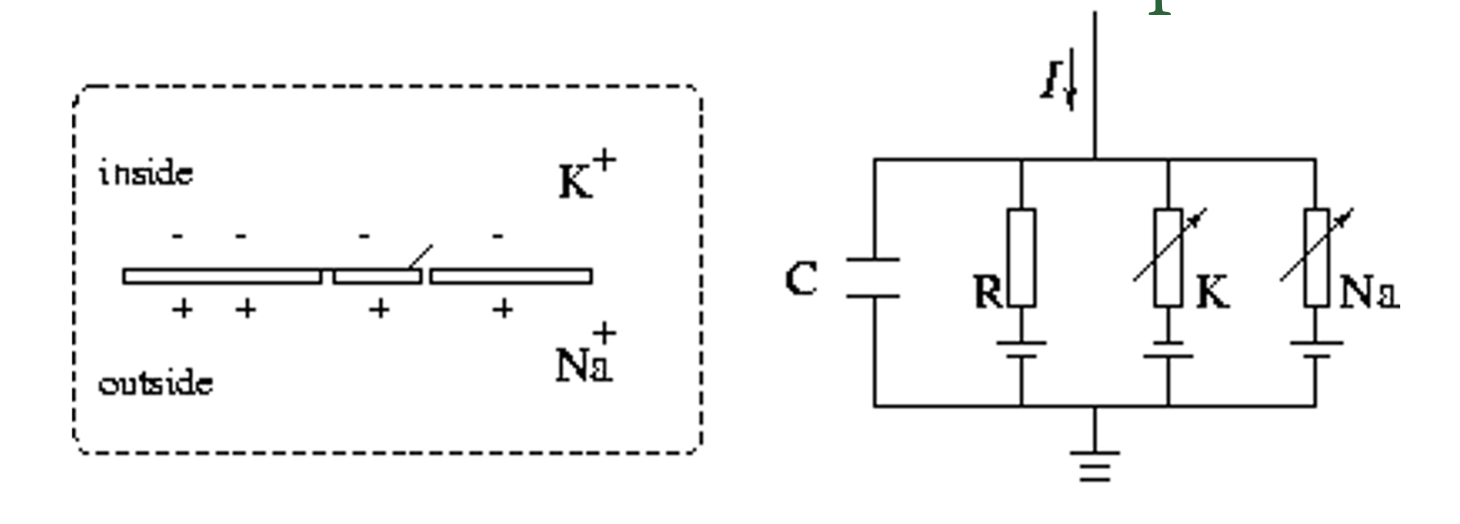
\includegraphics[keepaspectratio,alt={fig1}]{figures/fig1.png}}
\caption{fig1}
\end{figure}

    \textbf{Figura 1}. Comparación entre la membrana y la analogía a un
capacitor y el flujo de iones en analogía a baterías o canales de
corriente.

    \subsection{Problema}\label{problema}

En esta tarea se nos solicita realizar un código en algún lenguaje de
programación para reproducir, en la medida de lo posible, el mapa de
bifurcación de la \textbf{Figura B}, que representa las regiones de
activación para los parámetros del estímulo \(I_2\) y \(\Delta I_2\)
como se muestra en la \textbf{Figura A}.

En la región se varian diferentes valores de \(I_2 \in [0, 8]\) y
\(\Delta I_2 \in [0, 6]\). Y en cada punto de la región ocurren
diferentes impulsos formando trenes de picos en la región \(R\),
impulsos latentes en la región \(S\) y supresiones prontas en la región
\(I\).

    \begin{figure}
\centering
\pandocbounded{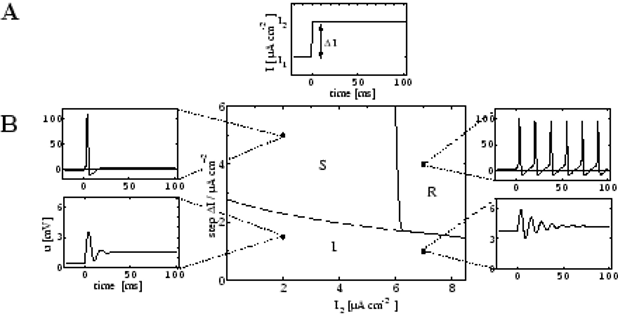
\includegraphics[keepaspectratio,alt={mapaHH}]{figures/mapa-hh.png}}
\caption{mapaHH}
\end{figure}

    \textbf{Figura 2}. (A) Función de impulso asociada al tiempo \(I(t)\) y
su diferencial \(\Delta I\). (B) Región entre los impulsos y su
diferencial, formando activaciones de tren \(R\), latentes \(S\) o
decadentes \(I\).

    \subsection{Ecuaciones de la Dinámica de
Hodkin-Huxley}\label{ecuaciones-de-la-dinuxe1mica-de-hodkin-huxley}

Basados en el modelo de corriente, los valores empíricos para las
conductancias \(g_x\), los potenciales inversos \(E_x\) y las funciones
\(\alpha_x(u)\) y \(\beta_x(u)\) con \(x = \{Na (n), K (m), L (h)\}\)
son:

\[
C_m \frac{d V}{d t} = -g_{Na} m^3 h (V - V_{Na}) - g_K n^4 (V - V_K) - g_L (V - V_L) + I
\]

\[
\frac{d m}{d t} = \alpha_m(u) \cdot (1 - m) - \beta_m(u) \cdot m
\]

\[
\frac{d n}{d t} = \alpha_n(u) \cdot (1 - n) - \beta_n(u) \cdot n
\]

\[
\frac{d h}{d t} = \alpha_h(u) \cdot (1 - h) - \beta_h(u) \cdot h
\]

Con los los valores empíricos reportados en la \textbf{Figura 3}.

    \begin{figure}
\centering
\pandocbounded{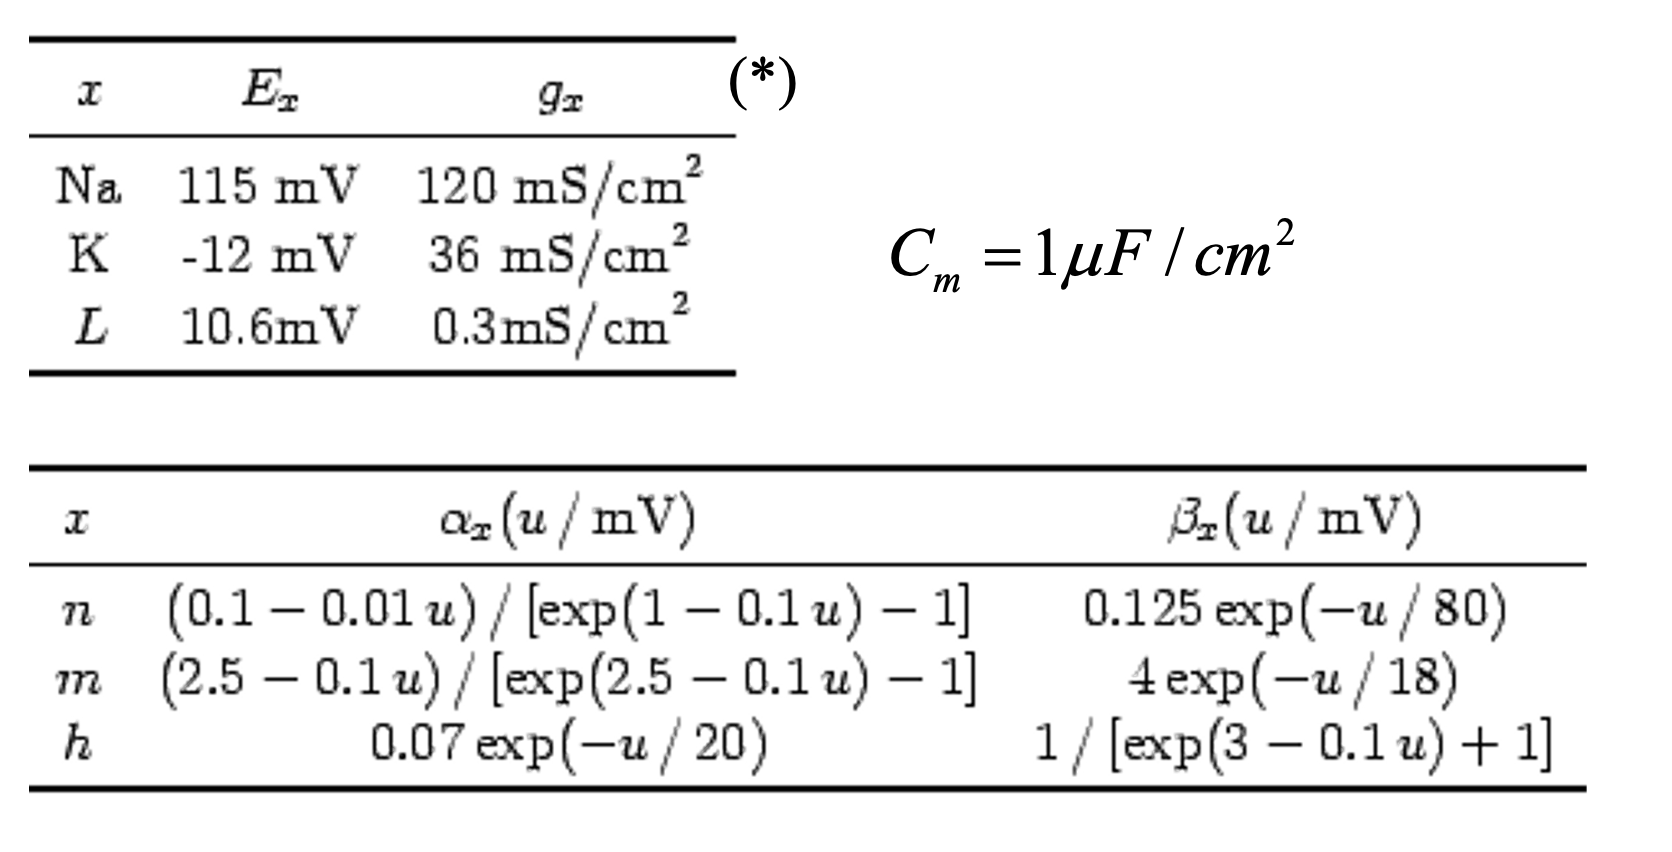
\includegraphics[keepaspectratio,alt={fig3}]{figures/fig3.png}}
\caption{fig3}
\end{figure}

    \textbf{Figura 3}. Valores empíricos reportados por Hodkin-Huxley para
las conductancias, potenciales reversos y las funciones \(\alpha_x(u)\)
y \(\beta_x(u)\).

(*) Referidos a un potencial de reposo cero.

En la norma actual, debe restarse -\(65 mV\) a los valores de \(E_x\)

    \section{Simulación}\label{simulaciuxf3n}

    Para resolver este problema, se desarrolló un simulador en \emph{Ruby}
resolviendo manualmente las ecuaciones diferenciales e implementando la
dinámica según los parámetros \(I_2\) y \(\Delta I_2\).

En el simulador podemos ver 3 regiones gráficas:

\begin{itemize}
\tightlist
\item
  \emph{Izquierda Arriba} - Muestra el potencial de la membrana generado
  por los parámetros que toman \(I_2\) y \(\Delta I\) mediante la
  solución de \(u(t)\).
\item
  \emph{Izquierda Abajo} - Muestra el impulso generado en el tiempo
  \(I(t)\)
\item
  \emph{Derecha} - Muestra una región seleccionable para tomar los
  valores de los parámetros \(I_2 \in [0, 8]\) y
  \(\Delta I_2 \in [0, 6]\).
\end{itemize}

Al pulsar sobre la región derecha, se lanzarán además 10 soluciones
aleatorias cercanas, para ir completando el mapa de las regiones.

El color de cada punto se calcula según el área bajo la curva medida
para el impulso.

Esto permite colorear del naranja al azul cuando el tren de picos
aumenta y el área bajo la curva crece.

    \subsection{Fase 1 - Impulsos bajos}\label{fase-1---impulsos-bajos}

En la región inferior izquierda, para cuando \(I_2 \approx 0\) y
\(\Delta I_2 \approx 0\) podemos observar cómo el impulso es corto y
decae inmediatamente, haciendo referencia a la región \(I\).

    \begin{figure}
\centering
\pandocbounded{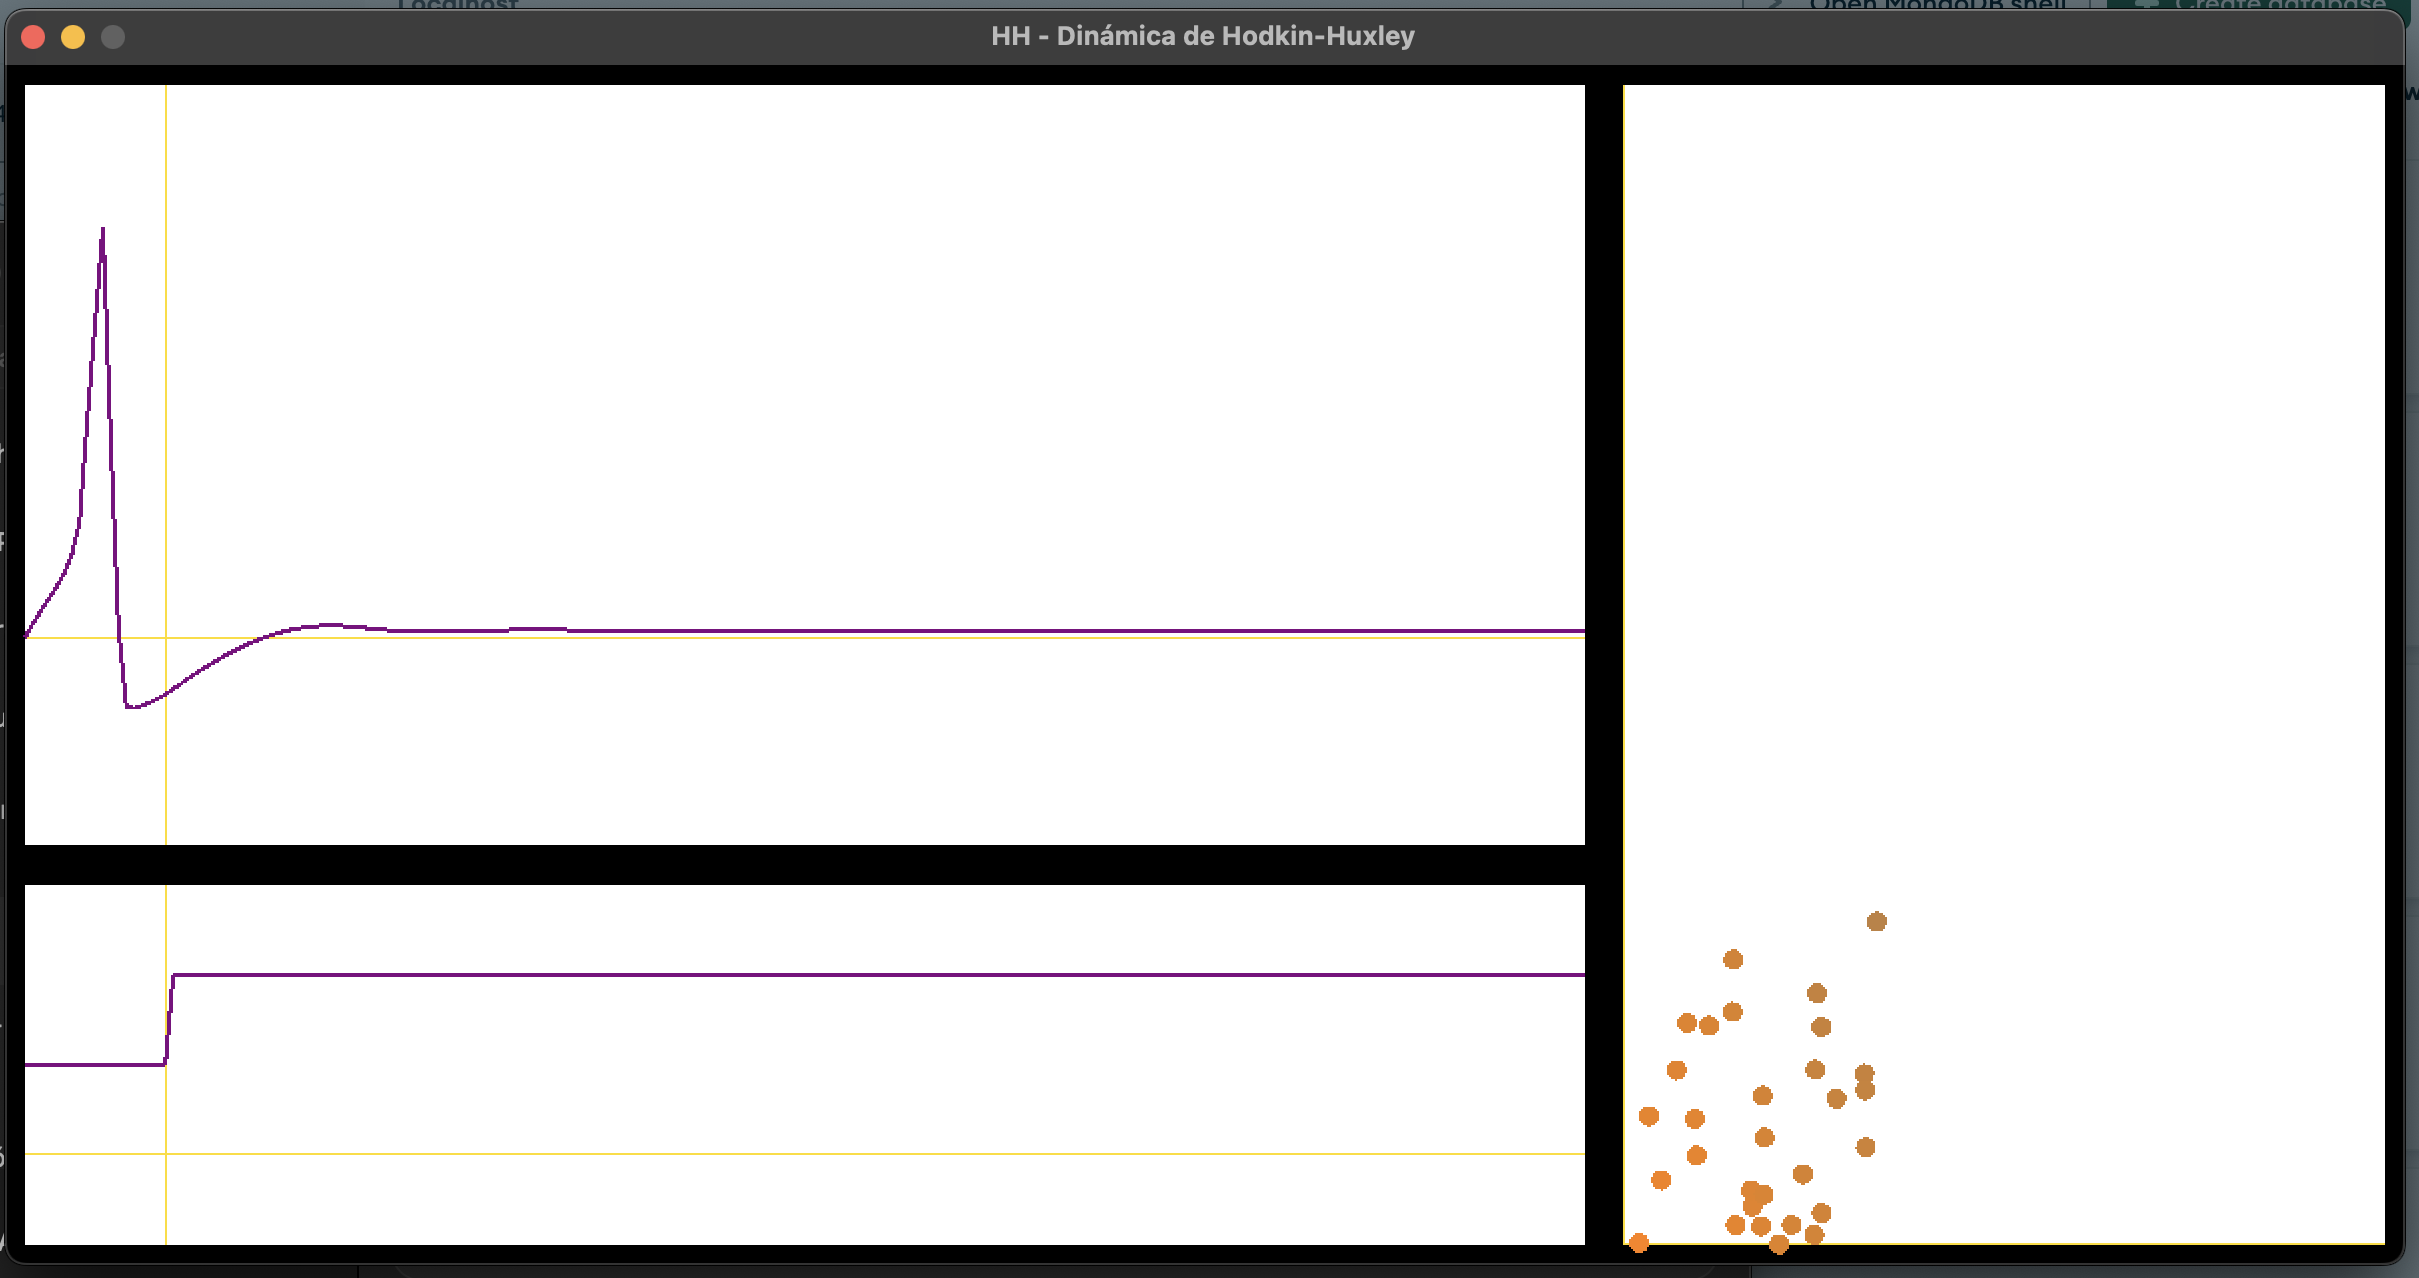
\includegraphics[keepaspectratio,alt={f1}]{figures/f1.png}}
\caption{f1}
\end{figure}

    \subsection{Fase 2 - Aumento de la cola de
impulsos}\label{fase-2---aumento-de-la-cola-de-impulsos}

Cuando en la región se aumenta a \(\Delta I_2\) y se mantiene a
\(I_2 \approx (0, 3)\) el comportamiento del impulso forma colas
parecidos a trenes que decaen rápidamente, haciendo referencia a la
región \(S\) y mostrando un color más ocre.

    \begin{figure}
\centering
\pandocbounded{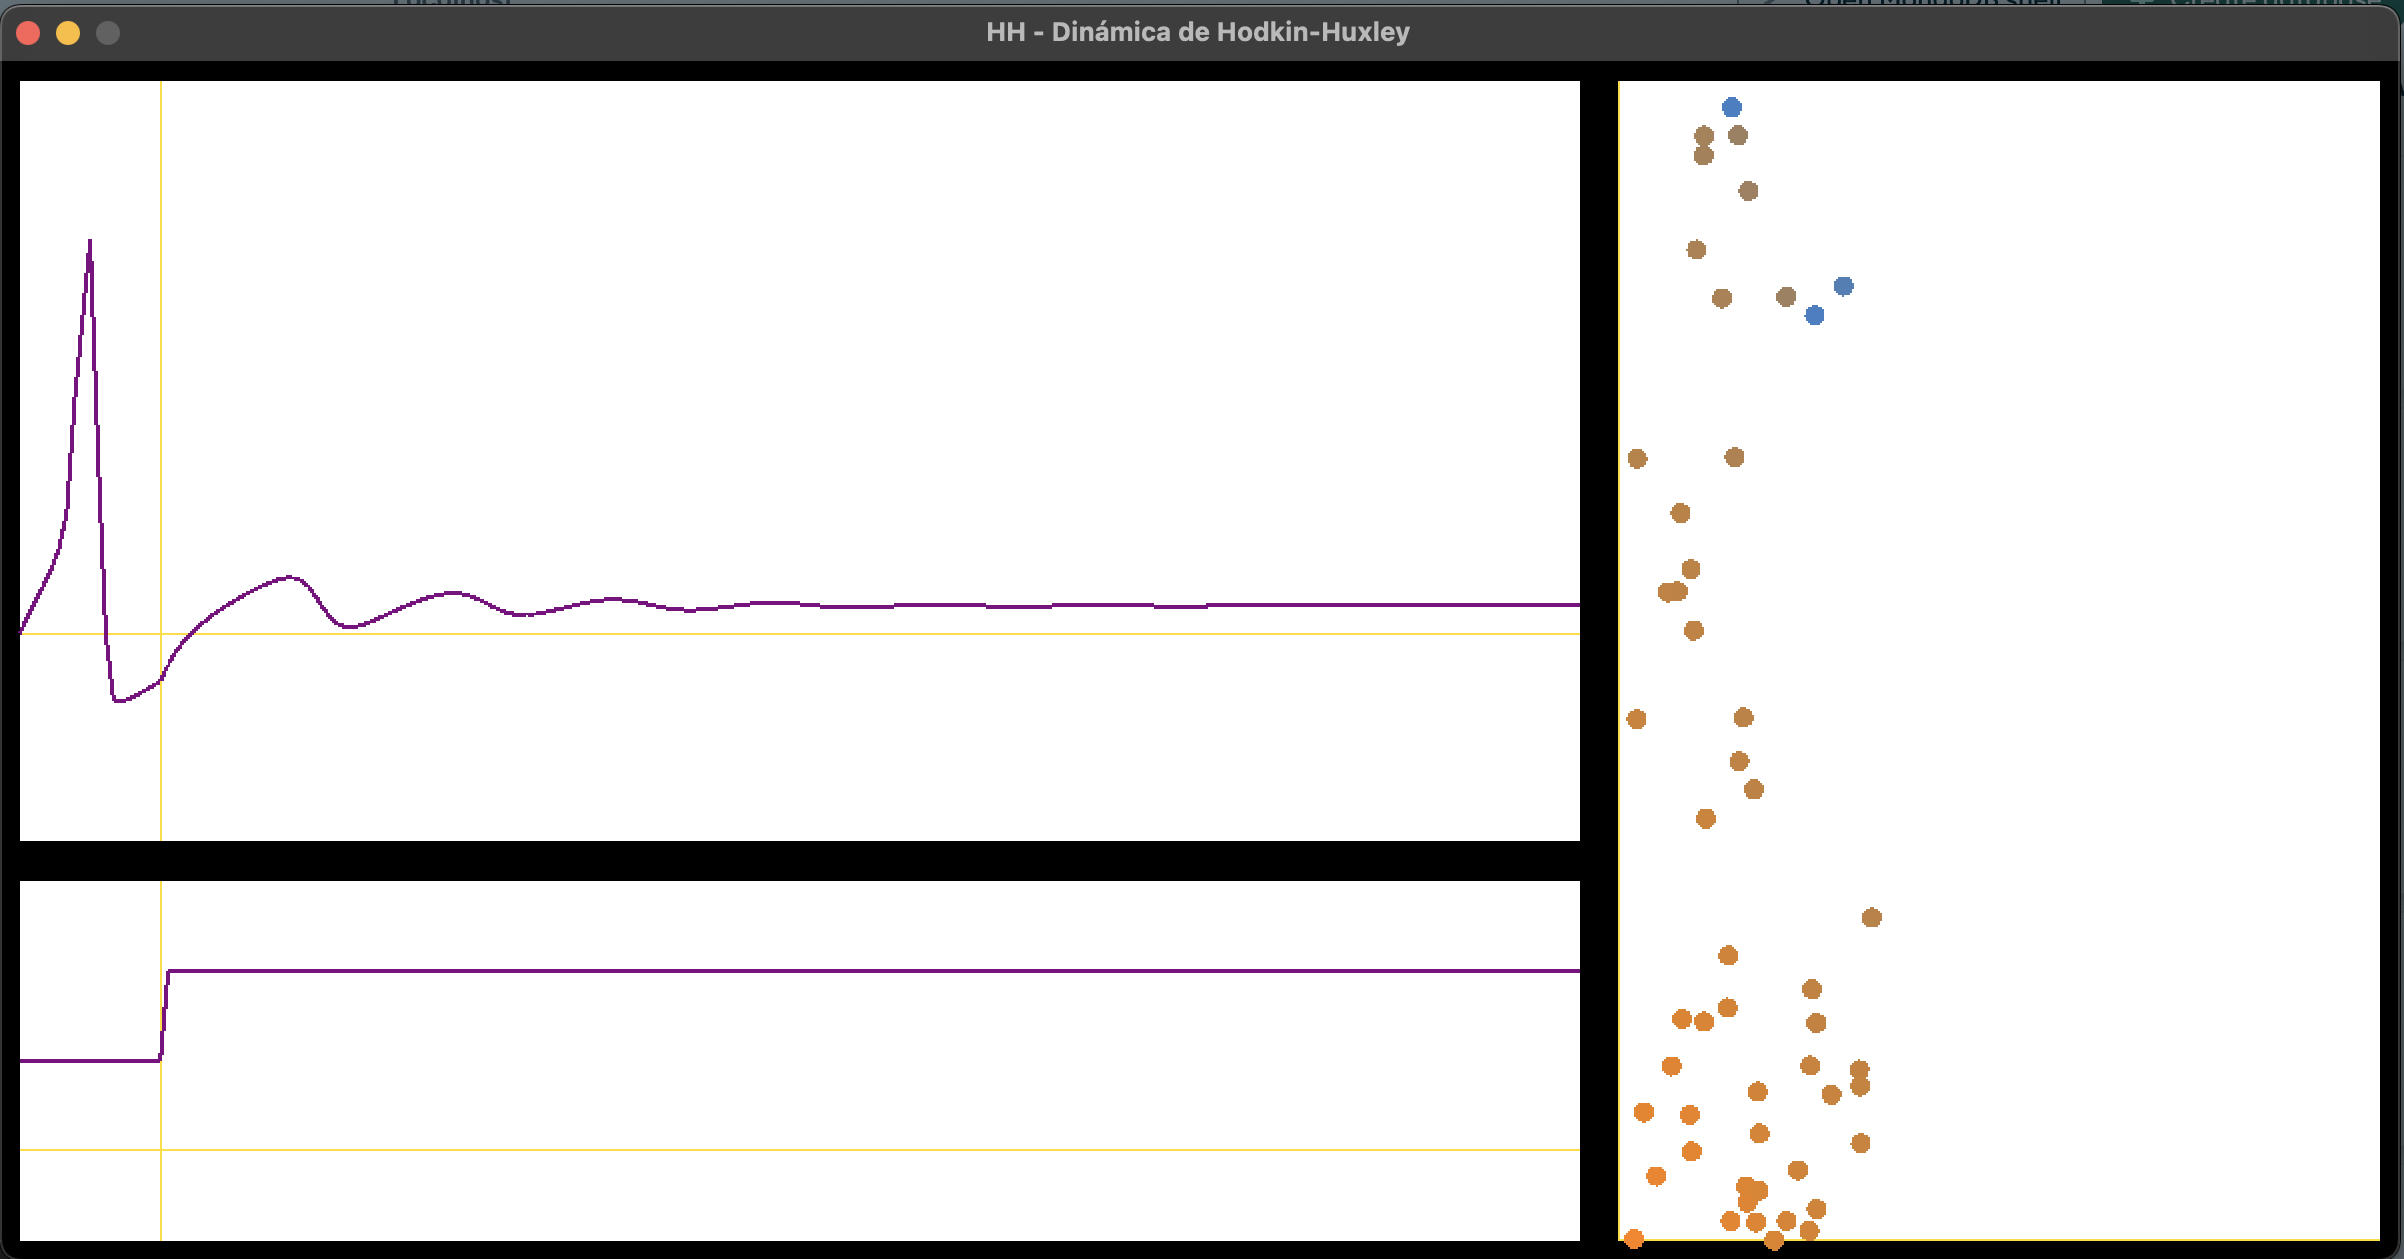
\includegraphics[keepaspectratio,alt={f3}]{figures/f3.png}}
\caption{f3}
\end{figure}

    \subsection{Fase 3 - Tren de picos}\label{fase-3---tren-de-picos}

Cuando \(\Delta I_2\) crece (\(\Delta I_2 \approx 6\)), los picos ya no
decaen formando así un tren de picos.

    \begin{figure}
\centering
\pandocbounded{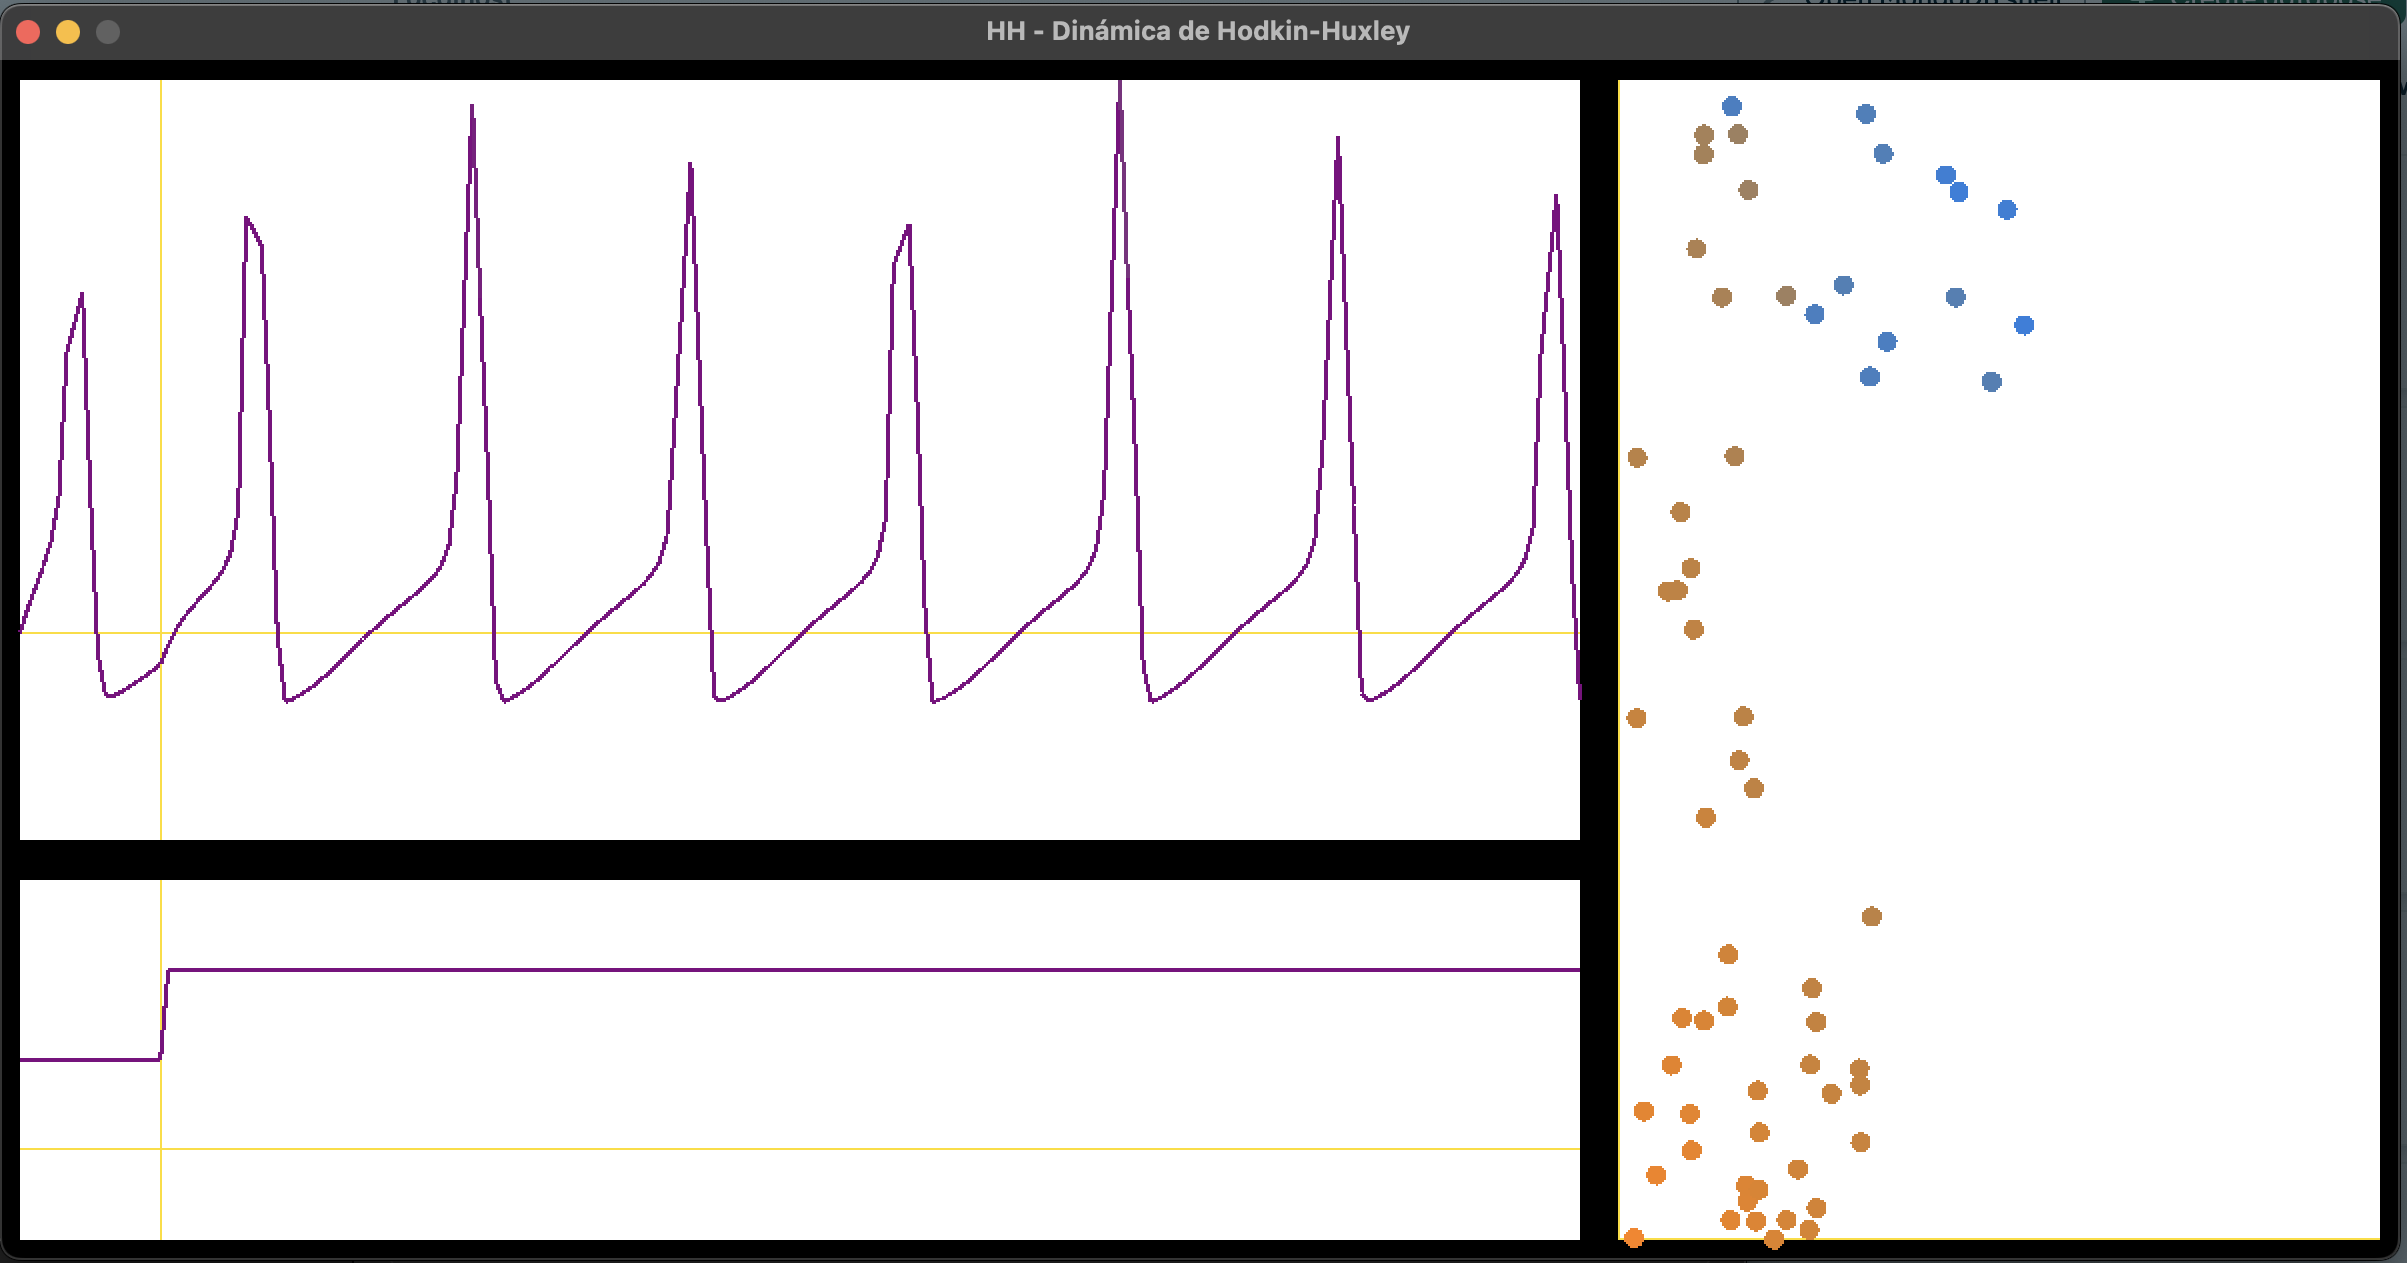
\includegraphics[keepaspectratio,alt={f4}]{figures/f4.png}}
\caption{f4}
\end{figure}

    \subsection{Región completa}\label{regiuxf3n-completa}

Con suficientes simulaciones se puede observar en qué puntos se
mantendrá el tren de picos y en cuáles decaerá, formando así un
comportamiento similar al reportado en el mapa de \(HH\).

    \begin{figure}
\centering
\pandocbounded{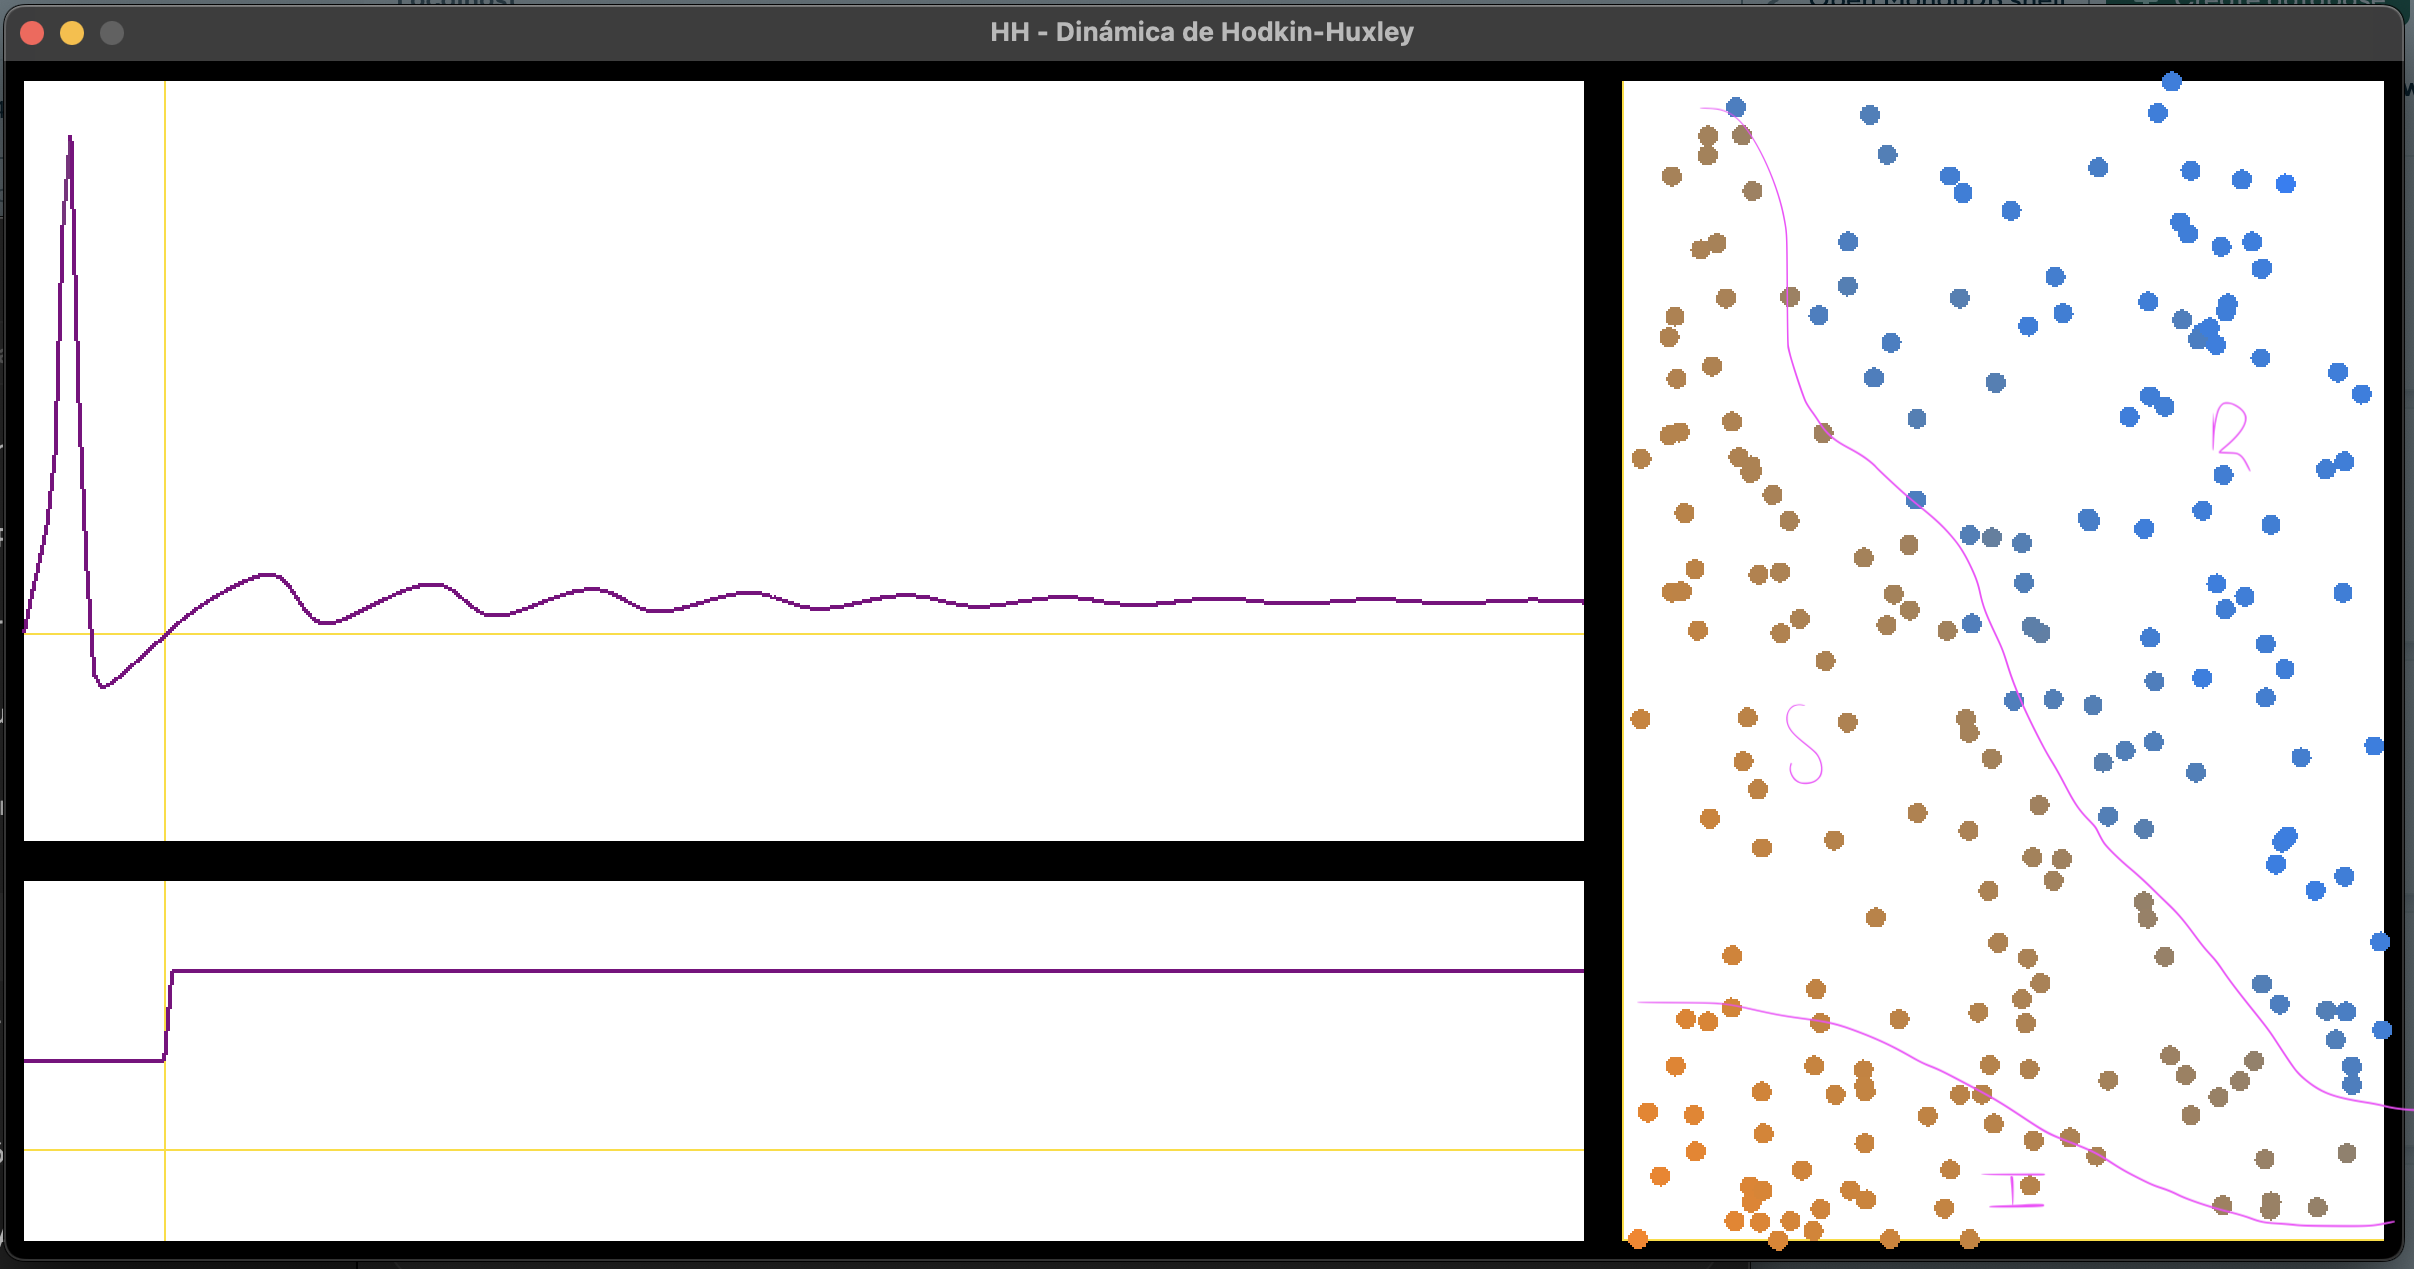
\includegraphics[keepaspectratio,alt={f6}]{figures/f6.png}}
\caption{f6}
\end{figure}

    \section{Conclusiones}\label{conclusiones}

En esta tarea hemos abordado un modelo que ha permitido el desarrollo de
las redes neuronales mediante mecanismos biológicos asimilados como
modelos eléctricos y ajustados empíricamente para producir activaciones
cortas y frecuentes.

Esto nos permite madurar el entendimiento de cómo los modelos
bioquímicos usan modelos matemáticos complicados y dinámicas complejas
para poder hacer intercambios de señales y energía mediante bombas y
depósitos de \(Na^+\) y \(K^+\), formando así instrumentos naturales
donde reside la inteligencia natural, que reconstruimos mediante modelos
matemáticos, para llegar a una inteligencia artificial.

    \section{Anexo}\label{anexo}

A continuación se deja el código del simulador desarrollado.

\begin{Shaded}
\begin{Highlighting}[]
\CommentTok{\# Universidad Autónoma Metropolitana}
\CommentTok{\# Unidad Iztapalapa}
\CommentTok{\# Maestría en Matemáticas Aplicadas e Industriales}
\CommentTok{\# Profesor: Joaquín Delgado Fernández}

\CommentTok{\# Alan Badillo Salas (alan@nomadacode.com)}
\CommentTok{\# Julio, 2025}

\CommentTok{\# Simulador de la Dinámica del Modelo de Hodkin{-}Huxley}

\FunctionTok{require} \VerbatimStringTok{\textquotesingle{}ruby2d\textquotesingle{}}
\FunctionTok{require\_relative} \VerbatimStringTok{\textquotesingle{}curve\_box\textquotesingle{}}

\VariableTok{$w} \OperatorTok{=} \DecValTok{800}
\VariableTok{$h} \OperatorTok{=} \DecValTok{400}

\NormalTok{set }\WarningTok{width:} \VariableTok{$w}
\NormalTok{set }\WarningTok{height:} \VariableTok{$h}
\NormalTok{set }\WarningTok{title:} \VerbatimStringTok{\textquotesingle{}Simulación 10 {-} Dinámica diferencial\textquotesingle{}}

\VariableTok{$t0} \OperatorTok{=} \OperatorTok{{-}}\DecValTok{3}
\VariableTok{$c} \OperatorTok{=} \DecValTok{1}
\VariableTok{$t1} \OperatorTok{=} \VariableTok{$t0} \OperatorTok{+} \VariableTok{$c}

\ControlFlowTok{def}\NormalTok{ impulso(t)}
\NormalTok{  (t }\OperatorTok{\textgreater{}=} \VariableTok{$t0} \OperatorTok{\&\&}\NormalTok{ t }\OperatorTok{\textless{}=} \VariableTok{$t1}\NormalTok{) }\OperatorTok{?} \FloatTok{1.0} \OperatorTok{:} \FloatTok{0.0}
\ControlFlowTok{end}

\NormalTok{curve1 }\OperatorTok{=} \DataTypeTok{CurveBox}\AttributeTok{.new}\NormalTok{(}
  \WarningTok{ox:} \DecValTok{10}\NormalTok{,}
  \WarningTok{oy:} \DecValTok{10}\NormalTok{,}
  \WarningTok{sx:} \DecValTok{380}\NormalTok{,}
  \WarningTok{sy:} \DecValTok{380}\NormalTok{,}
  \WarningTok{tmin:} \OperatorTok{{-}}\DecValTok{3}\NormalTok{,}
  \WarningTok{tmax:} \DecValTok{3}\NormalTok{,}
  \WarningTok{ymin:} \OperatorTok{{-}}\FloatTok{1.5}\NormalTok{,}
  \WarningTok{ymax:} \FloatTok{1.5}\NormalTok{,}
  \WarningTok{f:}\NormalTok{ method(}\WarningTok{:impulso}\NormalTok{)}
\NormalTok{)}

\CommentTok{\# dv/dt = {-}a v + b * impulso(t)}
\CommentTok{\# v(t + λt) = v(t) + λt * ({-}a v(t) + b * impulso(t))}


\VariableTok{$v} \OperatorTok{=} \FloatTok{0.0}   \CommentTok{\# Estado inicial}
\VariableTok{$a} \OperatorTok{=} \FloatTok{1.0}   \CommentTok{\# Decaimiento}
\VariableTok{$b} \OperatorTok{=} \FloatTok{2.0}   \CommentTok{\# Peso del impulso}
\VariableTok{$dt} \OperatorTok{=} \FloatTok{0.05} \CommentTok{\# Paso temporal}

\ControlFlowTok{def}\NormalTok{ dinamica(t)}
  \VariableTok{$v} \OperatorTok{+=} \VariableTok{$dt} \OperatorTok{*}\NormalTok{ (}\OperatorTok{{-}}\VariableTok{$a} \OperatorTok{*} \VariableTok{$v} \OperatorTok{+} \VariableTok{$b} \OperatorTok{*}\NormalTok{ impulso(t))}
  \VariableTok{$v}
\ControlFlowTok{end}

\NormalTok{curve2 }\OperatorTok{=} \DataTypeTok{CurveBox}\AttributeTok{.new}\NormalTok{(}
  \WarningTok{ox:} \DecValTok{410}\NormalTok{,}
  \WarningTok{oy:} \DecValTok{10}\NormalTok{,}
  \WarningTok{sx:} \DecValTok{380}\NormalTok{,}
  \WarningTok{sy:} \DecValTok{380}\NormalTok{,}
  \WarningTok{tmin:} \OperatorTok{{-}}\DecValTok{3}\NormalTok{,}
  \WarningTok{tmax:} \DecValTok{3}\NormalTok{,}
  \WarningTok{ymin:} \OperatorTok{{-}}\FloatTok{1.5}\NormalTok{,}
  \WarningTok{ymax:} \FloatTok{1.5}\NormalTok{,}
  \WarningTok{f:}\NormalTok{ method(}\WarningTok{:dinamica}\NormalTok{)}
\NormalTok{)}

\NormalTok{curve1}\AttributeTok{.draw}
\NormalTok{curve2}\AttributeTok{.draw}

\NormalTok{update }\ControlFlowTok{do}
  \VariableTok{$t0} \OperatorTok{+=} \FloatTok{0.01}
  \VariableTok{$t1} \OperatorTok{=} \VariableTok{$t0} \OperatorTok{+} \VariableTok{$c}

  \ControlFlowTok{if} \VariableTok{$t0} \OperatorTok{\textgreater{}} \DecValTok{3}
    \VariableTok{$t0} \OperatorTok{=} \OperatorTok{{-}}\DecValTok{3}
  \ControlFlowTok{end}

\NormalTok{  curve1}\AttributeTok{.draw}
\NormalTok{  curve2}\AttributeTok{.draw}
\ControlFlowTok{end}

\NormalTok{show}
\end{Highlighting}
\end{Shaded}


    % Add a bibliography block to the postdoc
    
    
    
\end{document}
